\documentclass[11pt]{article}

\usepackage[margin=1in]{geometry}
\usepackage[T1]{fontenc}
\usepackage[utf8]{inputenc}
\usepackage{lmodern}
\usepackage{microtype}
\usepackage{amsmath}
\usepackage{booktabs}
\usepackage{graphicx}
\usepackage{xcolor}
\usepackage[numbers]{natbib}
\usepackage[hidelinks]{hyperref}

\newcommand{\todo}[1]{\textcolor{red}{[TODO: #1]}}

\title{Neighbours Matter: A Simple Baseline for\\Budgeted Context Compaction of Long Conversations}
\author{Viraj Rana\\Independent Researcher\\\texttt{hackteck404@gmail.com}}
\date{}

\begin{document}
\maketitle

\begin{abstract}
When a conversation outgrows a language model's context window, some turns must be dropped.
We study this compaction step in isolation: given a long two-person conversation, a question,
and a word budget, select the turns to keep. We score compactors on LoCoMo by
\emph{evidence recall}, the share of the gold answer-bearing turns that survive compaction,
which needs no model in the loop. All settings are tuned on five conversations and reported on
the other five (776 questions). Keeping the most recent turns retains 2\% of the evidence at
500 words; BM25 retains 55\%, dense retrieval 71\%, and a BM25--dense hybrid 76\%. Adding to each
turn half the best score of its same-session neighbour, which captures the fact that an answer
is usually the reply to the turn that matches the question, raises this to 78\% at 500 words and
94\% at 4,000 words. The gain is large and reliable for lexical ranking (+4.9 to +7.2 points)
and small for the hybrid, where only the 500-word gain is distinguishable from zero under a
paired bootstrap. We also report a negative result: an entity-dependency graph that
keeps the turns a selected turn depends on helps on a synthetic suite built for it, but on
LoCoMo dev tuning switches it off. With Qwen2.5-7B answering from a 1,000-word compacted
context, the recall ordering carries over to answers: hybrid ranking reaches 62.4\% judge
accuracy against 50.9\% for BM25, 6.4\% for recency and 70.9\% for an oracle given only the gold
turns. Code and results are public.
\end{abstract}

\section{Introduction}

Chat assistants and agents accumulate long histories. Once a history exceeds the context window,
or simply costs too much to prefill, the system has to decide what to keep. The common defaults
are to truncate to the last $N$ messages or to summarise older turns. Both are blind to the
question being asked next, and both fail in a predictable way: an early turn that holds the
answer is the first thing to go.

Retrieval-based memory systems \citep{packer2023memgpt,chhikara2025mem0,zhong2024memorybank}
address this by fetching relevant past content at query time, but they bundle retrieval with
extraction, summarisation and LLM-based memory management, which makes it hard to tell what part
of the pipeline is responsible for what is kept. We isolate the selection step. A compactor sees
the full conversation, the next question and a word budget, and returns a subset of turns. We
measure only whether the turns that contain the answer survive.

This framing lets us ask a narrow question with a clean answer: under a fixed budget, how much
of the evidence do simple selection policies keep, and which ingredients matter? Our
contributions are:

\begin{itemize}
  \item A model-free evaluation of budgeted compaction on LoCoMo \citep{maharana2024locomo}
        with a strict dev/held-out split, comparing recency, summarisation-style keyword
        filtering, BM25, dense and hybrid ranking at four budgets.
  \item \emph{Neighbour smoothing}, a one-line change that adds to each turn a fraction of its
        best same-session neighbour's score. It is the only ingredient beyond the ranker that
        improves recall on LoCoMo; its benefit is large for lexical ranking and shrinks to a
        small, budget-dependent gain for a strong hybrid ranker.
  \item A negative result on entity-dependency repair: keeping the turns a selected turn
        depends on (via reused entities) rescues early constraints on a synthetic suite, but on
        real conversations entity reuse is too common to mark a dependency, and tuning disables
        it.
  \item An answer-accuracy check with an open 7B model showing that recall differences between
        rankers carry over to answers, and that the best compactor still trails an oracle
        context by 8.5 judge points.
\end{itemize}

\section{Related Work}

\paragraph{Long-term conversational memory.}
Multi-session chat datasets \citep{xu2022goldfish} and benchmarks such as LoCoMo
\citep{maharana2024locomo} and LongMemEval \citep{wu2025longmemeval} test whether models can use
facts stated many sessions earlier. Systems such as MemGPT \citep{packer2023memgpt},
MemoryBank \citep{zhong2024memorybank} and Mem0 \citep{chhikara2025mem0} manage an external
memory with LLM calls. We study the cheaper, model-free selection step that such systems, or a
plain chat application, can apply to the raw history.

\paragraph{Prompt and context compression.}
Token-level methods drop low-information tokens using a small language model
\citep{li2023selective,jiang2023llmlingua}. They operate below the turn level and need a model
at compaction time; our selectors work on whole turns with no model, or with only a sentence
embedder.

\paragraph{Retrieval.}
Our rankers are standard: BM25 \citep{robertson2009bm25}, a dense embedder
\citep{nussbaum2024nomic}, and a convex combination of min-max normalised scores
\citep{bruch2023fusion}, as in retrieval-augmented generation \citep{lewis2020rag}. Because
models use the middle of long contexts poorly \citep{liu2024lost}, keeping fewer but relevant
turns can matter even when everything would fit.

\section{Task and Evaluation}

A conversation is a sequence of turns $t_1,\dots,t_n$ grouped into sessions. Given a question
$q$ and a budget $B$ in words, a compactor returns a subset $S$ with $\sum_{t\in S}|t|\le B$.

\paragraph{Data.}
LoCoMo \citep{maharana2024locomo} has 10 two-person conversations of 369--689 turns
(9k--19k words) and about 2,000 questions, each annotated with the turns that hold its answer.
We drop adversarial (unanswerable) questions and questions whose evidence ids do not resolve to
a turn. Conversations 1--5 form the dev split (760 questions) and 6--10 the held-out split
(776 questions: 423 single-hop, 140 multi-hop, 165 temporal, 48 open-domain).

\paragraph{Metric.}
Evidence recall is $|E\cap S|/|E|$ for gold evidence turns $E$, averaged over questions. It
measures what the context keeps, independent of how well a particular model reads it. We
report it at $B\in\{500,1000,2000,4000\}$ words.

\paragraph{Protocol.}
Every hyperparameter (neighbour weight, hybrid mixing weight, entity document-frequency cap,
parent depth) was chosen on dev by best mean recall over the four budgets, then frozen. All
held-out numbers were computed once with those settings.

\section{Method}

All selectors share one greedy loop. Turns are ranked by a score; the best remaining turn is
added if it fits the remaining budget and skipped otherwise, until no turn fits. Selected turns
are presented in their original order.

\paragraph{Rankers.}
\emph{BM25} uses $k_1=1.5$, $b=0.75$ over lower-cased word tokens; \emph{BM25-stem} additionally
removes stopwords and strips common English suffixes. \emph{Dense} is cosine similarity with
\texttt{nomic-embed-text} \citep{nussbaum2024nomic}, using its document and query prefixes.
\emph{Hybrid} is $0.3\cdot\mathrm{mm}(s_{\text{BM25-stem}}) + 0.7\cdot\mathrm{mm}(s_{\text{dense}})$,
where $\mathrm{mm}$ is min-max normalisation over the conversation's turns.

\paragraph{Neighbour smoothing.}
In conversation the answer to a question is often the \emph{reply} to the turn that matches it
(``What breed is he?'' matches ``I got a new dog!''; the answer is in the next turn, ``Biscuit is
a corgi''). We therefore add to each turn a fraction $\alpha$ of the best score among its
immediate neighbours in the same session:
\[
  s'(t_i) = s(t_i) + \alpha \max\bigl(s(t_{i-1}),\, s(t_{i+1})\bigr),
\]
with neighbours from other sessions treated as score 0. Dev tuning gives $\alpha=0.5$ for
BM25-stem and the hybrid and $\alpha=0.25$ for dense.

\paragraph{Entity-dependency repair.}
We build a graph with an edge from the turn that first mentions an entity to each later turn
that reuses it, ignoring speaker names and entities that occur in more than a fraction
$\tau$ of turns. When a turn is selected, its ancestors up to depth $d$ are added too; if they do
not fit whole, each is folded into a one-line pin. On synthetic data, back-reference cues
(``as I said'', ``that limit'') also create edges to earlier constraint-like turns.

\paragraph{Baselines.}
\emph{last-$N$} keeps the most recent turns that fit. \emph{sum-drop} spends about two thirds of
the budget on the most recent turns and the rest (at most 40 words) on eight-word extractive
pins of older turns that contain a digit or a constraint keyword (``limit'', ``rule'',
``must'', \dots); only whole kept turns count towards recall. \emph{Overlap scorer} is our first
version, tuned on the synthetic suite: per-word value of query-word overlap plus recency plus a
bonus for constraint-like turns, minus redundancy with already kept turns, with entity repair.

\section{Results}

\begin{figure*}[t]
  \centering
  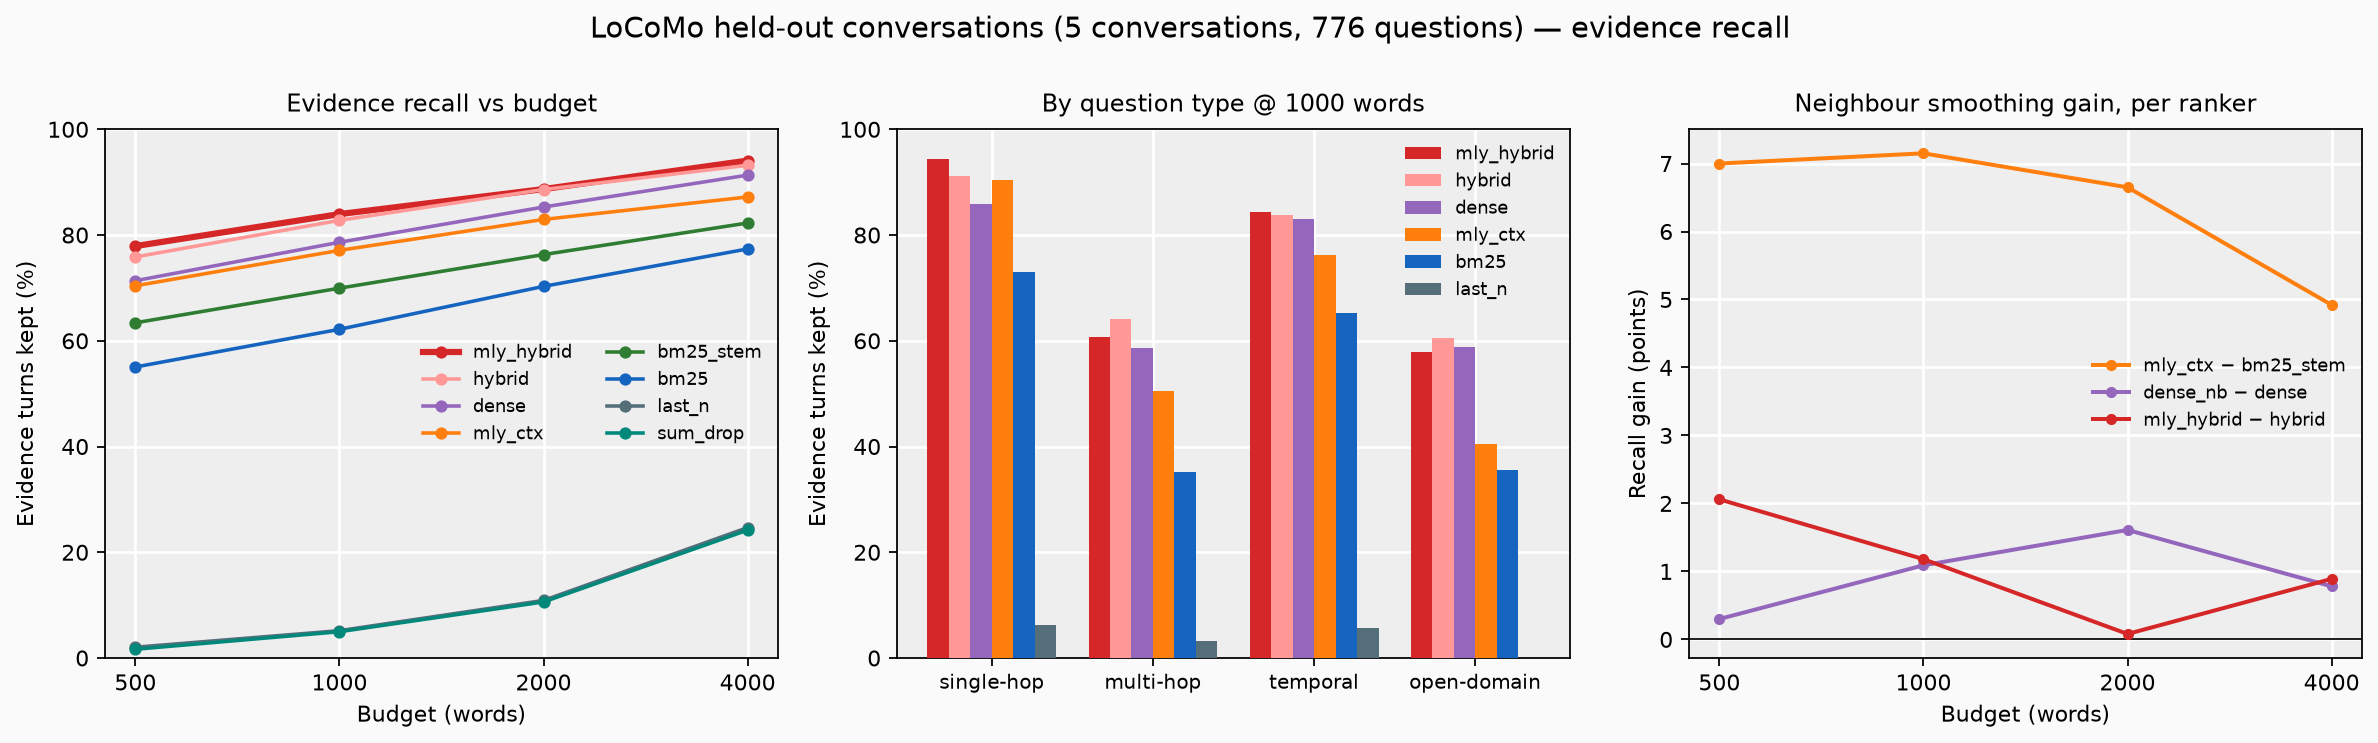
\includegraphics[width=\textwidth]{locomo.png}
  \caption{Held-out evidence recall on LoCoMo (776 questions). Left: recall versus budget.
  Middle: by question type at 1,000 words. Right: gain from neighbour smoothing for each ranker.}
  \label{fig:locomo}
\end{figure*}

\begin{table}[t]
  \centering
  \small
  \begin{tabular}{lrrrrr}
    \toprule
    Method & 500 & 1000 & 2000 & 4000 & MH@4000 \\
    \midrule
    Hybrid + neighbour      & \textbf{77.9} & \textbf{84.0} & \textbf{88.7} & \textbf{94.1} & \textbf{85.3} \\
    Hybrid                  & 75.9 & 82.8 & 88.6 & 93.2 & \textbf{85.3} \\
    Dense + neighbour       & 71.7 & 79.7 & 86.9 & 92.1 & 82.5 \\
    Dense                   & 71.4 & 78.6 & 85.3 & 91.3 & 82.6 \\
    BM25-stem + neighbour   & 70.4 & 77.1 & 83.0 & 87.2 & 69.1 \\
    BM25-stem               & 63.4 & 70.0 & 76.3 & 82.3 & 62.9 \\
    BM25                    & 55.0 & 62.2 & 70.3 & 77.4 & 57.0 \\
    BM25 + repair ($\tau{=}0.005$, $d{=}1$) & 54.1 & 61.6 & 70.8 & 78.0 & 59.4 \\
    BM25 + repair ($\tau{=}0.02$, $d{=}2$)  & 50.1 & 59.3 & 68.6 & 77.5 & 61.6 \\
    Overlap scorer (v1)     & 5.6  & 9.8  & 19.3 & 37.5 & --- \\
    last-$N$                & 2.0  & 5.2  & 10.9 & 24.7 & --- \\
    sum-drop                & 1.6  & 5.0  & 10.6 & 24.2 & --- \\
    \bottomrule
  \end{tabular}
  \caption{Held-out evidence recall (\%) by budget in words; MH is the multi-hop subset
  (140 questions). Paired-bootstrap intervals for the key differences are in
  Table~\ref{tab:boot}.}
  \label{tab:main}
\end{table}

\begin{table}[t]
  \centering
  \small
  \begin{tabular}{lrrrr}
    \toprule
    Difference & 500 & 1000 & 2000 & 4000 \\
    \midrule
    Hybrid + nb $-$ hybrid   & \textbf{+2.1} {\scriptsize[0.3, 3.9]} & +1.2 {\scriptsize[$-$0.3, 2.7]} & +0.1 {\scriptsize[$-$1.2, 1.3]} & +0.9 {\scriptsize[$-$0.2, 2.0]} \\
    BM25-stem + nb $-$ BM25-stem & \textbf{+7.0} {\scriptsize[5.0, 9.0]} & \textbf{+7.2} {\scriptsize[5.1, 9.2]} & \textbf{+6.7} {\scriptsize[4.9, 8.5]} & \textbf{+4.9} {\scriptsize[3.3, 6.7]} \\
    Dense + nb $-$ dense     & +0.3 {\scriptsize[$-$1.3, 1.9]} & +1.1 {\scriptsize[$-$0.2, 2.5]} & \textbf{+1.6} {\scriptsize[0.5, 2.7]} & \textbf{+0.8} {\scriptsize[0.0, 1.6]} \\
    Hybrid $-$ dense         & \textbf{+4.5} {\scriptsize[2.3, 6.7]} & \textbf{+4.2} {\scriptsize[2.3, 6.1]} & \textbf{+3.3} {\scriptsize[2.0, 4.7]} & \textbf{+1.9} {\scriptsize[0.8, 3.0]} \\
    \bottomrule
  \end{tabular}
  \caption{Held-out recall differences (points) with 95\% paired-bootstrap intervals over the
  776 questions (10,000 resamples). Bold: interval excludes zero. nb = neighbour smoothing.}
  \label{tab:boot}
\end{table}

\subsection{Evidence recall}

Table~\ref{tab:main} and Figure~\ref{fig:locomo} show the held-out results. Recency and
keyword policies keep under 25\% of the evidence even at 4,000 words: in LoCoMo the answer to a
question is usually many sessions old. The ranker matters most. Dense retrieval beats every
lexical variant, including stemmed BM25 with neighbour smoothing, and is far ahead on multi-hop
questions (82.6 vs.\ 69.1 at 4,000 words). The hybrid improves on dense by 1.9 to 4.5 points.
Hybrid ranking with neighbour smoothing is best at every budget. Dev showed the same ordering
(mean over budgets 88.2 for hybrid + neighbour, 86.6 for hybrid, 84.4 for dense).

\subsection{Neighbour smoothing}

Smoothing adds 4.9 to 7.2 points to stemmed BM25, 0.3 to 1.6 to dense, and 0.1 to 2.1 to the
hybrid (Figure~\ref{fig:locomo}, right). The better the ranker, the less a neighbour adds:
a dense embedder already scores a reply as related to the question even when it shares no
words with it. Table~\ref{tab:boot} makes this concrete: the gain on stemmed BM25 is clearly
non-zero at every budget, but on the hybrid only the 500-word gain (+2.1, interval 0.3 to 3.9)
excludes zero; at 1,000 to 4,000 words the hybrid with and without smoothing are statistically
indistinguishable on this data. The intervals resample questions as if independent; questions
from the same conversation are correlated, so they are, if anything, too narrow.

The gain is not uniform across question types (Table~\ref{tab:cats}). For the hybrid it comes
entirely from single-hop questions (+6.2 points at 500 words, 423 questions). Smoothing loses 7
of the 16 type-by-budget cells, mostly multi-hop and open-domain at small budgets: when evidence
is spread over several distant turns, budget spent on neighbours is budget not spent on the
next distant hit.

\begin{table}[t]
  \centering
  \small
  \begin{tabular}{lrrrr}
    \toprule
    Type ($n$) & 500 & 1000 & 2000 & 4000 \\
    \midrule
    Single-hop (423)  & 84.9 / \textbf{91.1} & 91.1 / \textbf{94.4} & 95.2 / \textbf{96.3} & 98.1 / \textbf{98.8} \\
    Multi-hop (140)   & \textbf{52.5} / 48.2 & \textbf{64.2} / 60.8 & \textbf{74.8} / 74.4 & 85.3 / 85.3 \\
    Temporal (165)    & \textbf{79.9} / 78.7 & 83.7 / \textbf{84.4} & \textbf{89.4} / 87.1 & 92.2 / \textbf{93.7} \\
    Open-domain (48)  & \textbf{50.1} / 45.8 & \textbf{60.5} / 57.9 & 68.0 / \textbf{68.9} & 76.3 / \textbf{79.4} \\
    \bottomrule
  \end{tabular}
  \caption{Held-out recall (\%) by question type: hybrid / hybrid + neighbour smoothing.}
  \label{tab:cats}
\end{table}

\subsection{Entity-dependency repair: a negative result}

Repair is the mechanism this work started from, and it does not help on LoCoMo. With neighbour
smoothing in place, dev tuning selects a document-frequency cap of $\tau=0.002$. With 369--689
turns per conversation, that admits only entities that occur in at most one turn, so the graph
has \emph{no edges} in any of the 10 conversations, and recall is identical to the same selector
without repair, to the last reported digit, on both splits. Where repair is active
(plain BM25; $\tau=0.005$ gives 0--113 edges per conversation, $\tau=0.02$ gives 177--543), it is
a trade-off: within a point overall, +4.6 on multi-hop at 4,000 words with depth 2, and about
$-5$ at 500 words. Entities in casual conversation (``work'', ``family'', ``trip'') recur too
often for reuse to signal that a later turn depends on an earlier one.

On a synthetic suite built around this failure (24 template dialogues, 12 held out, in which a
rule stated early is asked about much later), repair is what makes the difference: at a
55-token budget the rule survives in 100\% of held-out dialogues with repair, 33\% without it,
and 17\% for last-$N$. A keyword-based summary baseline also reaches 100\% there, because its
keywords happen to match the rules, and fails on LoCoMo for the same reason. The suite shows
that the mechanism works when dependencies are real and sparse; LoCoMo shows that it does not
transfer to open-domain chat.

\subsection{Answer accuracy}

To check that recall differences carry over to answers, we give each compactor's 1,000-word
context, grouped by session and headed with the session date, to Qwen2.5-7B
\citep{qwen2024qwen25} at temperature 0, ask for a short answer, and score it against the gold
answer with SQuAD-style token F1 \citep{rajpurkar2016squad} and a CORRECT/WRONG verdict from the
same model acting as judge \citep{zheng2023judge}. The \emph{oracle} context contains only the
gold evidence turns (63 words on average).

\begin{table}[t]
  \centering
  \small
  \begin{tabular}{lrrrrr}
    \toprule
    Method & Recall & F1 & J & J (MH) & J (temp.) \\
    \midrule
    Oracle (gold turns only) & 100.0 & 57.0 & 70.9 & 75.0 & 49.1 \\
    Hybrid + neighbour       & 84.0 & \textbf{52.5} & \textbf{62.4} & \textbf{55.0} & \textbf{35.8} \\
    Hybrid                   & 82.8 & 52.0 & \textbf{62.4} & \textbf{55.0} & \textbf{35.8} \\
    BM25-stem + neighbour    & 77.1 & 50.3 & 59.0 & 49.3 & 31.5 \\
    BM25                     & 62.2 & 41.9 & 50.9 & 40.7 & 27.3 \\
    last-$N$                 & 5.2  & 5.3  & 6.4  & 10.0 & 4.2 \\
    \bottomrule
  \end{tabular}
  \caption{Held-out answer quality with Qwen2.5-7B at a 1,000-word budget (776 questions):
  evidence recall, token F1 and LLM-judge accuracy J (\%), overall and for multi-hop (140) and
  temporal (165) questions.}
  \label{tab:qa}
\end{table}

Table~\ref{tab:qa} shows that the recall ordering carries over. The hybrid rankers beat BM25 by
11.5 judge points (95\% paired-bootstrap interval 8.1 to 14.8) and stemmed BM25 with smoothing
by 3.4 (0.3 to 6.6). Keeping the last turns is nearly useless. Neighbour smoothing on top of the
hybrid does not change answer quality at this budget: +0.6 F1 ($-$1.2 to 2.3) and exactly the
same judge accuracy, from 53 questions that only the smoothed context answers correctly and 53
that only the unsmoothed one does. This matches Table~\ref{tab:boot}, where its recall gain at
1,000 words is not distinguishable from zero.

Compaction still costs accuracy: the oracle is 8.5 judge points above the best compactor
(5.0 to 12.0), although that compactor keeps 84\% of the evidence. Missing evidence is not the
only cost: the oracle's 63-word context carries no distractors, while a 1,000-word context is
mostly unrelated turns. Temporal questions are hard even for the oracle (49.1), because their
gold answers are absolute dates the model must compute from relative expressions and session
dates.

\subsection{Cost}

Selection is cheap. With turn embeddings computed once per conversation and cached, the hybrid
selector with smoothing takes about 6\,ms per question on a CPU; BM25 takes about 3\,ms. The
lexical selectors need no model at all. These timings exclude embedding the question and the
turns.

\section{Limitations}

Evidence recall measures what survives, not whether a model answers correctly; the
answer-accuracy experiment uses a single 7B model at a single budget, and the same model
serves as judge. The judge is lenient: it accepts partial answers to list questions (``rock
climbing'' for ``rock climbing, fishing, camping''), so judge accuracy overstates exact
correctness, though it does so for every method alike. Answers are generated at temperature 0,
but GPU inference is not bit-exact: in an accidental double run, 135 of 2,302 repeated answers
differed in wording, which moved aggregate scores by at most 0.5 points. LoCoMo has only 10
conversations, generated by LLM-based agents and then edited by human annotators rather than
collected from real users, so the held-out split is five conversations, and differences of a point or two should be read with the intervals in
Table~\ref{tab:boot}. Budgets are counted in whitespace-separated words rather than model tokens. We compare
selection policies only; we do not compare against full memory systems that extract or
summarise with an LLM. The synthetic suite was written by us around the failure that
dependency repair targets and is evidence for the mechanism, not for generalisation.

\section{Conclusion}

For budgeted compaction of long conversations, the ranker does most of the work: a BM25--dense
hybrid keeps 76\% of the evidence at 500 words where recency keeps 2\%. Adding a fraction of the
neighbouring turn's score costs nothing and helps lexical rankers a lot; on a strong hybrid
ranker it helps only at the tightest budget. Tracking
entity dependencies between turns, which motivated this work, rescues early constraints in
controlled dialogues but does not help on real conversations. We release the code, results and
evaluation scripts to make compaction policies easy to compare.

\section*{Reproducibility}
Code, per-setting results and plotting scripts are at
\url{https://github.com/Viraj-rana/ctx-compact}. LoCoMo is distributed under CC BY-NC 4.0 and is
downloaded by a script rather than redistributed. All experiments run locally; the dense
methods and the answer-accuracy run use Ollama with \texttt{nomic-embed-text} and
\texttt{qwen2.5:7b}.

\section*{Acknowledgements}
The author used an AI coding assistant for parts of the implementation, the analysis scripts
and drafting this paper. All experiments, numbers and claims were checked by the author, who
takes full responsibility for the content.

\bibliographystyle{plainnat}
\bibliography{refs}

\end{document}
